\documentclass{jsarticle}
\usepackage[dvipdfmx]{graphicx}
\usepackage{listings}
\usepackage{afterpage}
\begin{document}
\title{課題1ダウンサンプリング}
\author{13EC060 武澤 裕介}
\maketitle
\begin{abstract}
まずmatlabを用いて画像のダウンサンプリングを行い画像の変化について考察する。また応用として補完方法をtriangleに変更してその違いについて考察する。
\end{abstract}
\section{補完オプション「box」の場合}
まず、今回使用する原画像を図1に示す。
\begin{lstlisting}[basicstyle=\ttfamily\footnotesize, frame=single]
filename = uigetfile('*');
ORG=imread(filename); % 原画像の入力
imagesc(ORG); axis image; % 画像の表示
 \end{lstlisting}
を用いてまず原画像を表示させる。
\begin{figure}[htbp]
 \begin{center}
  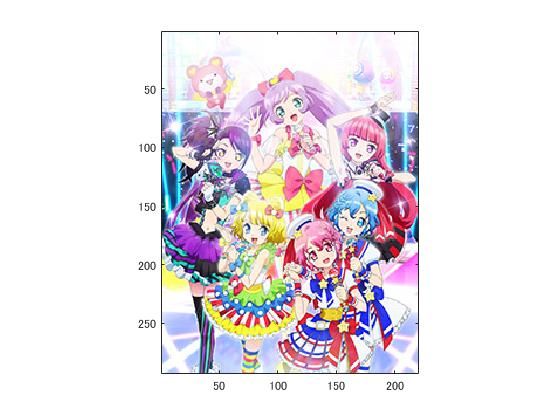
\includegraphics[width=10cm]{kadai1-0.jpg}
 \end{center}
 \caption{原画像}
\end{figure}

次に1/2サンプリングを行う。まず、原画像の大きさを1/2にし、その後2倍に拡大すれば良い。図2に1/2サンプリング後の画像を示す。

\begin{lstlisting}[basicstyle=\ttfamily\footnotesize, frame=single]
IMG = imresize(ORG,0.5); % 画像の縮小
IMG2 = imresize(IMG,2,'box'); % 画像の拡大
 \end{lstlisting}
とすれば1/2サンプリング後の画像が表示される

\begin{figure}[htbp]
 \begin{center}
  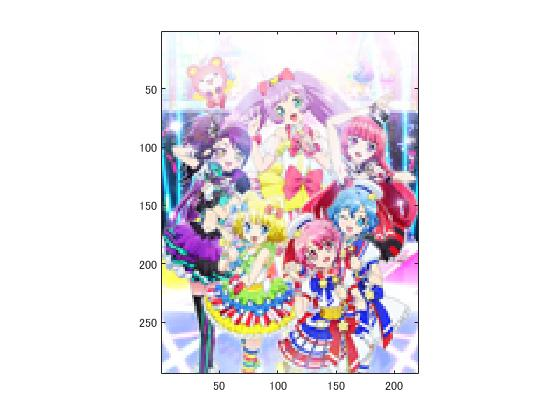
\includegraphics[width=10cm]{kadai1-1.jpg}
 \end{center}
 \caption{1/2サンプリング画像[box]}
\end{figure}

同様に原画像を1/4サンプリングするには,さらに画像を1/2倍に縮小した後,4倍に拡大すればよい.すなわち,

\begin{lstlisting}[basicstyle=\ttfamily\footnotesize, frame=single]
IMG = imresize(ORG,0.5); % 画像の縮小
IMG2 = imresize(IMG,4,'box'); % 画像の拡大
 \end{lstlisting}

とする.1/4サンプリングの結果を図3に示す.

\begin{figure}[htbp]
 \begin{center}
  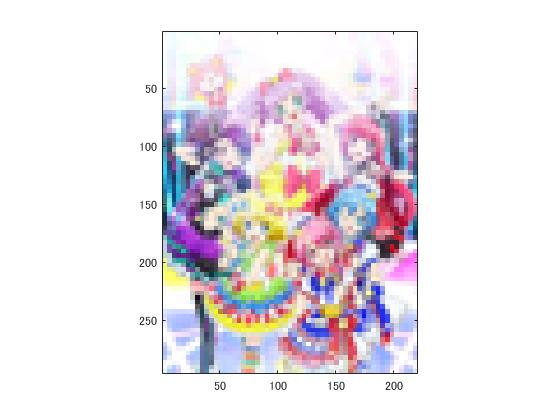
\includegraphics[width=10cm]{kadai1-2.jpg}
 \end{center}
 \caption{1/4サンプリング画像[box]}
\end{figure}

1/8から1/32サンプリングは,

\begin{lstlisting}[basicstyle=\ttfamily\footnotesize, frame=single]
IMG = imresize(ORG,0.5); % 画像の縮小
IMG2 = imresize(IMG,8,'box'); % 画像の拡大
 \end{lstlisting}

\begin{lstlisting}[basicstyle=\ttfamily\footnotesize, frame=single]
IMG = imresize(ORG,0.5); % 画像の縮小
IMG2 = imresize(IMG,16,'box'); % 画像の拡大
 \end{lstlisting}

\begin{lstlisting}[basicstyle=\ttfamily\footnotesize, frame=single]
IMG = imresize(ORG,0.5); % 画像の縮小
IMG2 = imresize(IMG,32,'box'); % 画像の拡大
 \end{lstlisting}

を行えばよい.サンプリングの結果を図4~6に示す.

\begin{figure}[htbp]
 \begin{center}
  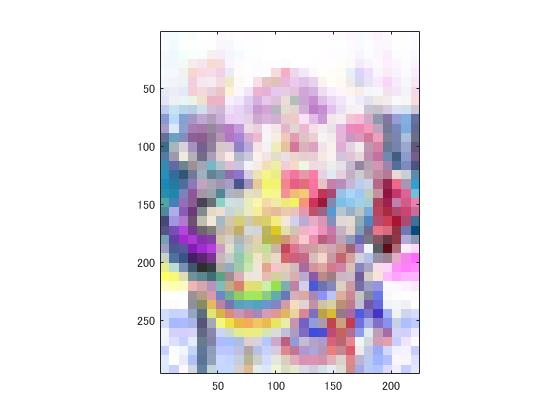
\includegraphics[width=10cm]{kadai1-3.jpg}
 \end{center}
 \caption{1/8サンプリング画像[box]}
 \begin{center}
  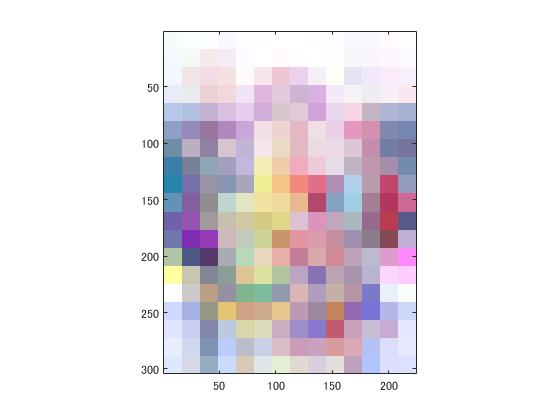
\includegraphics[width=10cm]{kadai1-4.jpg}
 \end{center}
 \caption{1/16サンプリング画像[box]}
\end{figure}

\begin{figure}[htbp]
 \begin{center}
  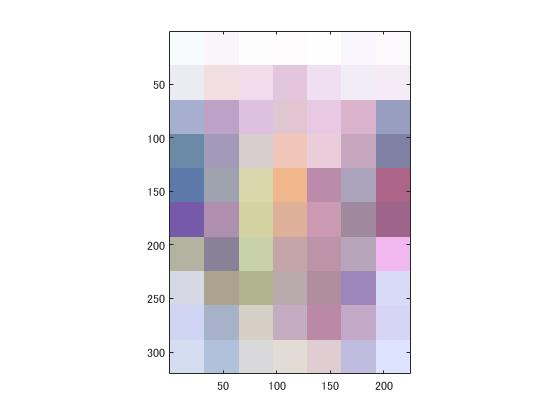
\includegraphics[width=10cm]{kadai1-5.jpg}
 \end{center}
 \caption{1/32サンプリング画像[box]}
\end{figure}

\clearpage
\section{補完オプション「triangle」の場合}
次に補完オプションを「triangle」としてダウンサンプリングしていく。1/2、1/4、1/8、1/16、1/32サンプリングそれぞれ以下のように表示する。

\begin{lstlisting}[basicstyle=\ttfamily\footnotesize, frame=single]
IMG = imresize(ORG,0.5); % 画像の縮小
IMG2 = imresize(IMG,2,'triangle'); % 画像の拡大
 \end{lstlisting}

\begin{lstlisting}[basicstyle=\ttfamily\footnotesize, frame=single]
IMG = imresize(ORG,0.5); % 画像の縮小
IMG2 = imresize(IMG,4,'triangle'); % 画像の拡大
 \end{lstlisting}

\begin{lstlisting}[basicstyle=\ttfamily\footnotesize, frame=single]
IMG = imresize(ORG,0.5); % 画像の縮小
IMG2 = imresize(IMG,8,'triangle'); % 画像の拡大
 \end{lstlisting}

\begin{lstlisting}[basicstyle=\ttfamily\footnotesize, frame=single]
IMG = imresize(ORG,0.5); % 画像の縮小
IMG2 = imresize(IMG,16,'triangle'); % 画像の拡大
 \end{lstlisting}

\begin{lstlisting}[basicstyle=\ttfamily\footnotesize, frame=single]
IMG = imresize(ORG,0.5); % 画像の縮小
IMG2 = imresize(IMG,32,'triangle'); % 画像の拡大
 \end{lstlisting}

\begin{figure}[htbp]
 \begin{center}
  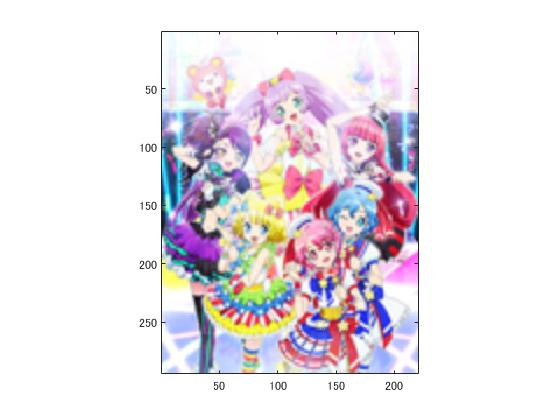
\includegraphics[width=10cm]{kadai1t-1.jpg}
 \end{center}
 \caption{1/2サンプリング画像[triangle]}
 \begin{center}
  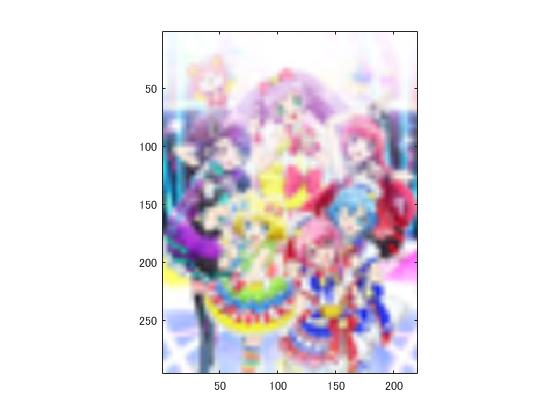
\includegraphics[width=10cm]{kadai1t-2.jpg}
 \caption{1/4サンプリング画像[triangle]}
 \end{center}
\end{figure}

 
\begin{figure}[htbp] 
 \begin{center}
  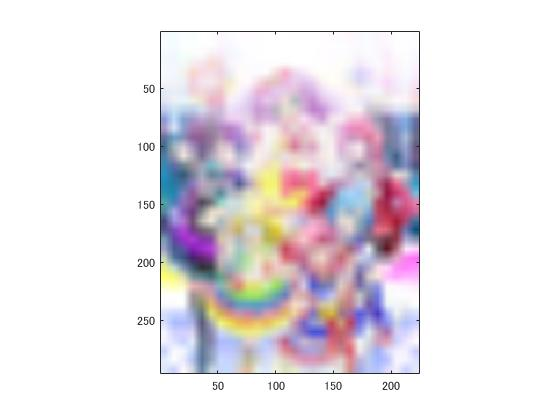
\includegraphics[width=10cm]{kadai1t-3.jpg}
 \end{center}
 \caption{1/8サンプリング画像[triangle]}
 \begin{center}
  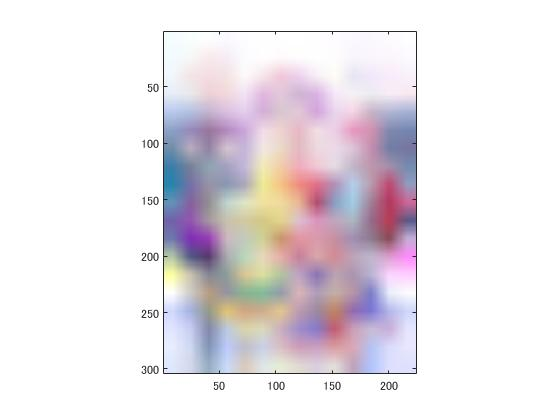
\includegraphics[width=10cm]{kadai1t-4.jpg}
 \end{center}
 \caption{1/16サンプリング画像[triangle]}
\end{figure}

\begin{figure}[htbp] 
\begin{center}
  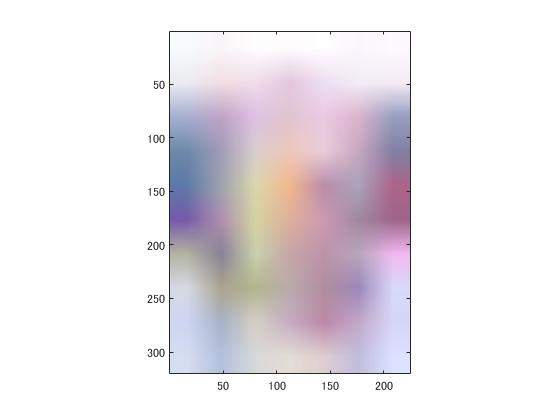
\includegraphics[width=10cm]{kadai1t-5.jpg}
 \end{center}
 \caption{1/32サンプリング画像[triangle]}
\end{figure}
\clearpage
\section{考察}
まず、今回補完のプロパティを「box」としてダウンサンプリングを行った場合、ブロックひずみが起きていることが図3、4、5、6で観察できる。
これに対して補完のプロパティを「triangle」とした場合、補完のプロパティを「box」とした場合とひずみ方が変わっているのが図8、9、10、11から観測できる。
これは、ダウンサンプリングにて欠損した画素の補完方法を決めているのが補完のプロパティであるが、使った補完プロパティが異なったからである。
\end{document}